\documentclass{standalone}

\usepackage{tikz}
\usetikzlibrary{calc}

% https://latexcolor.com/
\definecolor{darkolivegreen}{rgb}{0.33, 0.42, 0.18}
\definecolor{burntumber}{rgb}{0.54, 0.2, 0.14}

\begin{document}

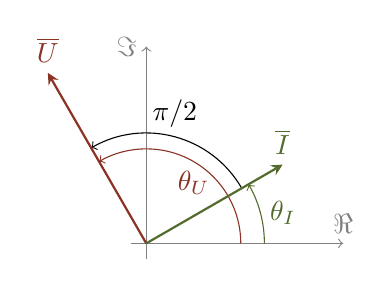
\begin{tikzpicture}
  \draw[->, thin, color=gray] (-0.2,0) -- (2.5,0) node[above] {$\Re$};
  \draw[->, thin, color=gray] (0,-0.2) -- (0,2.5) node[left] {$\Im$};

  \draw [->, thin, color=darkolivegreen](1.5,0)  arc[radius = 1.5, start angle= 0, end angle= 30] node [pos=0.5, right] {$\theta_I$};
  \draw [->, thin, color=burntumber](1.2,0)  arc[radius = 1.2, start angle= 0, end angle= 120] node [pos=0.5, below] {$\theta_U$};
  \draw [->, thin, color=black](30:1.4)  arc[radius = 1.4, start angle= 30, end angle= 120] node [pos=0.5, above] {$\pi/2$};
  \draw[->, >=stealth, thick, color = burntumber] (0, 0) -- (120:2.5) node[above] {$\overline{U}$};
  \draw[->, >=stealth, thick, color = darkolivegreen] (0, 0) -- (30:2) node[above] {$\overline{I}$};
\end{tikzpicture}

\end{document}


